%%%%%%%%%%%%%%%%%%%%%%%%%%%%%%%%%%%%%%%%%
% Programming/Coding Assignment
% LaTeX Template
%
% This template has been downloaded from:
% http://www.latextemplates.com
%
% Original author:
% Ted Pavlic (http://www.tedpavlic.com)
%
% Note:
% The \lipsum[#] commands throughout this template generate dummy text
% to fill the template out. These commands should all be removed when 
% writing assignment content.
%
% This template uses a Perl script as an example snippet of code, most other
% languages are also usable. Configure them in the "CODE INCLUSION 
% CONFIGURATION" section.
%
%%%%%%%%%%%%%%%%%%%%%%%%%%%%%%%%%%%%%%%%%

%----------------------------------------------------------------------------------------
%	PACKAGES AND OTHER DOCUMENT CONFIGURATIONS
%----------------------------------------------------------------------------------------

\documentclass{article}

\usepackage{fancyhdr} % Required for custom headers
\usepackage{lastpage} % Required to determine the last page for the footer
\usepackage{extramarks} % Required for headers and footers
\usepackage[usenames,dvipsnames]{color} % Required for custom colors
%\usepackage{graphicx}% % Required to insert images
\usepackage{listings} % Required for insertion of code
\usepackage{courier} % Required for the courier font
 \usepackage[pdftex]{graphicx}
  \graphicspath{{figures/}}
   \DeclareGraphicsExtensions{.pdf,.jpg,.png}
  \usepackage[caption=false,font=footnotesize]{subfig}
%\usepackage[cmex10]{amsmath}
\usepackage{amsmath,amssymb}
\interdisplaylinepenalty=2500
\usepackage{afterpage}
\newcommand\blankpage{%
    \null
    \thispagestyle{empty}%
    \addtocounter{page}{-1}%
    \newpage}


% Margins
\topmargin=-0.45in
\evensidemargin=0in
\oddsidemargin=0in
\textwidth=6.5in
\textheight=9.0in
\headsep=0.25in

\linespread{1.1} % Line spacing

% Set up the header and footer
\pagestyle{fancy}
\lhead{\hmwkAuthorName} % Top left header
%\chead{\hmwkClass\ (\hmwkClassInstructor\ \hmwkClassTime): \hmwkTitle} % Top center head
\rhead{\firstxmark} % Top right header
\lfoot{\lastxmark} % Bottom left footer
\cfoot{} % Bottom center footer
\rfoot{Page\ \thepage\ of\ \protect\pageref{LastPage}} % Bottom right footer
\renewcommand\headrulewidth{0.4pt} % Size of the header rule
\renewcommand\footrulewidth{0.4pt} % Size of the footer rule

\setlength\parindent{0pt} % Removes all indentation from paragraphs

%----------------------------------------------------------------------------------------
%	CODE INCLUSION CONFIGURATION
%----------------------------------------------------------------------------------------
%
\usepackage{listings}
\usepackage{color}

\definecolor{dkgreen}{rgb}{0,0.6,0}
\definecolor{gray}{rgb}{0.5,0.5,0.5}
\definecolor{mauve}{rgb}{0.58,0,0.82}

\lstset{frame=tb,
  language=C++,
  aboveskip=3mm,
  belowskip=3mm,
  showstringspaces=false,
  columns=flexible,
  basicstyle={\small\ttfamily},
  numbers=none,
  numberstyle=\tiny\color{gray},
  keywordstyle=\color{blue},
  commentstyle=\color{dkgreen},
  stringstyle=\color{mauve},
  breaklines=true,
  breakatwhitespace=true,
  tabsize=3
}


%----------------------------------------------------------------------------------------
%	DOCUMENT STRUCTURE COMMANDS
%	Skip this unless you know what you're doing
%----------------------------------------------------------------------------------------

%% Header and footer for when a page split occurs within a problem environment
\newcommand{\enterProblemHeader}[1]{
\nobreak\extramarks{#1}{#1 continued on next page\ldots}\nobreak
\nobreak\extramarks{#1 (continued)}{#1 continued on next page\ldots}\nobreak
}

% Header and footer for when a page split occurs between problem environments
\newcommand{\exitProblemHeader}[1]{
\nobreak\extramarks{#1 (continued)}{#1 continued on next page\ldots}\nobreak
\nobreak\extramarks{#1}{}\nobreak
}

\setcounter{secnumdepth}{0} % Removes default section numbers
\newcounter{homeworkProblemCounter} % Creates a counter to keep track of the number of problems
\setcounter{homeworkProblemCounter}{0}
\newcommand{\homeworkProblemName}{}
\newenvironment{homeworkProblem}[1][Section \arabic{homeworkProblemCounter}]{ % Makes a new environment called homeworkProblem which takes 1 argument (custom name) but the default is "Problem #"
\stepcounter{homeworkProblemCounter} % Increase counter for number of problems
\renewcommand{\homeworkProblemName}{#1} % Assign \homeworkProblemName the name of the problem
\section{\homeworkProblemName} % Make a section in the document with the custom problem count
\enterProblemHeader{\homeworkProblemName} % Header and footer within the environment
}{
\exitProblemHeader{\homeworkProblemName} % Header and footer after the environment
}

\newcommand{\problemAnswer}[1]{ % Defines the problem answer command with the content as the only argument
\noindent\framebox[\columnwidth][c]{\begin{minipage}{0.98\columnwidth}#1\end{minipage}} % Makes the box around the problem answer and puts the content inside
}

\newcommand{\homeworkSectionName}{}
\newenvironment{homeworkSection}[1]{ % New environment for sections within homework problems, takes 1 argument - the name of the section
\renewcommand{\homeworkSectionName}{#1} % Assign \homeworkSectionName to the name of the section from the environment argument
\subsection{\homeworkSectionName} % Make a subsection with the custom name of the subsection
\enterProblemHeader{\homeworkProblemName\ [\homeworkSectionName]} % Header and footer within the environment
}{
\enterProblemHeader{\homeworkProblemName} % Header and footer after the environment
}

%----------------------------------------------------------------------------------------
%	NAME AND CLASS SECTION
%----------------------------------------------------------------------------------------

\newcommand{\hmwkTitle}{Coursework \#1} % Assignment title
\newcommand{\hmwkDueDate}{Friday,\ March 18,\ 2016} % Due date
\newcommand{\hmwkClass}{MPHYG002} % Course/class
\newcommand{\hmwkAuthorName}{Maria Ruxandra Robu} % Your name

%----------------------------------------------------------------------------------------
%	TITLE PAGE
%----------------------------------------------------------------------------------------

\title{
\vspace{2in}
\textmd{\textbf{\hmwkClass:\ \hmwkTitle}}\\
\normalsize\vspace{0.1in}\small{Due\ on\ \hmwkDueDate}\\
%\vspace{0.1in}\large{\textit{\hmwkClassInstructor\ \hmwkClassTime}
\vspace{3in}
}

\author{\textbf{\hmwkAuthorName  - 14042500}}
\date{} % Insert date here if you want it to appear below your name

%----------------------------------------------------------------------------------------

\begin{document}

\maketitle

%----------------------------------------------------------------------------------------
%	TABLE OF CONTENTS
%----------------------------------------------------------------------------------------

%\setcounter{tocdepth}{1} % Uncomment this line if you don't want subsections listed in the ToC

%\newpage
%\tableofcontents
\newpage

This coursework implements the Iterative Closest Point (ICP) algorithm in two steps. The Point Based Task outputs a least squares estimation of the transformation between two given point clouds. The Surface Based Task takes as input two point sets with no assumption on the pair correspondence. However, an essential assumption with ICP is that there is a good initial alignment between the points. So, this algorithm iteratively minimizes the error:\\

\begin{equation}
RMS(R,t) = \sum_{i=1}^{n} || p_i - R  q_i - t ||^2
\end{equation}

ICP overview - Given two point clouds $p$ and $q$:
\begin{itemize}
  \item for each $q \in \{q\}_M$ find the closest match in $\{p\}_N$
  \item reject bad pairs (optional)
  \item get the least squares estimation of the transform $T = [R | t]$
  \begin{itemize}
 	 \item center the point clouds at their origin by subtracting their means
 	 \item compute the covariance matrix $C$ of the centered $ \tilde{p}$ and $ \tilde{q}$ 
 	 \item extract $R$ from the singular value decomposition of $C$ ( $R = U V'$ )
  	 \item the translation vector is $t = \bar{p} - R \bar{q}$
  \end{itemize}
  \item apply the current transformation $q_i = R q_i + t$ and start from the beginning
\end{itemize} 

This implementation of the algorithm stops iterating when the RMS stops decreasing. So, if the difference between two consecutive errors is less than a threshold, the algorithm is considered to have converged.\\

All of the tasks have been implemented in one stand-alone project and their documentation is structured in five sections. Hence, the implementation and design choices are detailed in Section 1. The second section goes over the basic error checking and the testing implemented with Catch. Sections 3 and 4 illustrate the usage of the entry points for Point Based and Surface Based Registration, respectively. Finally, section 5 discusses the application of ICP in medical imaging.

\clearpage
%----------------------------------------------------------------------------------------
%	PROBLEM 1
%----------------------------------------------------------------------------------------

% To have just one problem per page, simply put a \clearpage after each problem

\begin{homeworkProblem}

\textbf{Least Squares Estimation  and Surface Based Registration - Implementation}\\

The project is structured in the main classes: PointCloud, ICPRegistration and ExceptionICP. See Fig. \ref{fig:umlDiagram} for a UML diagram of the project. All of the functions and classes were built in the namespace ICP\_MPHYG02, to avoid any name clashes with other libraries. 

Whenever we have a point set, a new PointCloud object is created. The points are kept in a dynamic matrix from the Eigen library, which is efficient for big point clouds. New objects can be created by reading the input from a file or from another matrix. The copy constructor and assignment operator have been implemented as well. \\

The data is read from the file given a flag:
\begin{itemize}
	\item POINT\_BASED\_FLAG  for having one point per line (x y z)
	\item SURFACE\_BASED\_FLAG  for having 3 points per line (x1 y1 z1 x2 y2 z2 x3 y3 z3)
\end{itemize}  

The reading was made robust by using std::stringstream, which allows easy conversion between data types and store the coordinates as doubles. Furthermore, it is not dependent on a specific spacing between the numbers. A problem encountered in the beginning was that the reader was storing empty lines as 0s in the matrix, leading to point clouds of different sizes. So, in the current implementation, all of the empty lines are skipped.\\

ICPRegistration serves as a class that handles both tasks of this coursework. It contains defaults for the main parameters of ICP such that the instantiation is easier for the user. The flags used for reading from files in the initialization of PointClouds are used as inputs for the ICP solver. The default is the surface based algorithm since it is more general and it makes no assumptions regarding the point correspondences.

\begin{lstlisting}[language=c++]
ICPRegistration(bool ICP_FLAG = SURFACE_BASED_FLAG,
            int maxIter = 30,
            float errorThresh = 0.000001,
            float filterBadCorresp = 0.5);
\end{lstlisting}

All of the methods of ICPRegistration receive as parameters two PointCloud objects that correspond to the fixed and moving point sets. Since the PointCloud class has implemented methods such as applyTransformation() and getCenteredPCD(), this choice makes the code easier to follow and less prone to error. \\

In order to avoid calling the methods sequentially in a specific order to get the final matrix transform, the ICPRegistration class has the method solve(). Based on the flag set for the solver object, this method calls the appropriate algorithm for either point based or surface based registration and it outputs the RMS error and the final transformation matrix. In a more complex setting with more parameters and more methods, a Builder pattern could be used for this class.

\begin{lstlisting}[language=c++]
void solve(PointCloud& pFixedPCD,
            PointCloud& qMovingPCD,
            double& out_err,
            Eigen::Matrix4d& out_transfMatrix,
            std::string& outputPath);
\end{lstlisting}


%%%%%%%%%%%%%%%%%%%%%%%%%%%%%%%%%%%%%%%%
\begin{figure*}[!h]
\centering
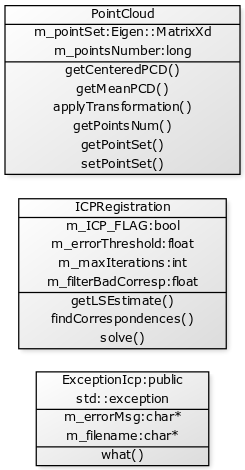
\includegraphics[height=4in]{umlDiagram}%
\caption{UML Diagram of the project class design}
\label{fig:umlDiagram}
\end{figure*}
%%%%%%%%%%%%%%%%%%%%%%%%%%%%%%%%%%%%%%%%

The Eigen library was heavily used in the implementation of these algorithms. Features like the dynamic allocation of matrices, advanced initialization (MatrixXd::Zero() or MatrixXd::Identity()), block operations (easy access to specific rows or columns of blocks of values inside a matrix) make it attractive for working with big matrices of data. Plus, reductions are broadcasting were used in the computation of the least squares estimation. The Eigen solver efficiently computes the singular value decomposition, which was used for the estimation of the rotation matrix. In conclusion, the use of Eigen makes the code easier to read and provides efficient and fast computation of matrix and linear algebra operations, ideal for problems with a high number of data points.

\end{homeworkProblem}
\clearpage
%\clearpage
%----------------------------------------------------------------------------------------
%	PROBLEM 2
%----------------------------------------------------------------------------------------

\begin{homeworkProblem}
\textbf{Error checking and Testing with Catch}\\

An exception class (ExceptionICP) was created to deal with all the errors raised during the execution of the ICP algorithm, which are then caught in the main entry point of the program. Given that the ExceptionICP class is derived from std::exception, the specific exceptions of the ICP program will be caught with:

\begin{lstlisting}[language=c++]
try
	{
		...
	 }
catch(std::exception& err)
	{
		...
	 }
\end{lstlisting}

See Fig. \ref{fig:exceptionEx} for an example of an exception thrown for an empty input file.

%%%%%%%%%%%%%%%%%%%%%%%%%%%%%%%%%%%%%%%%
\begin{figure*}[!h]
\centering
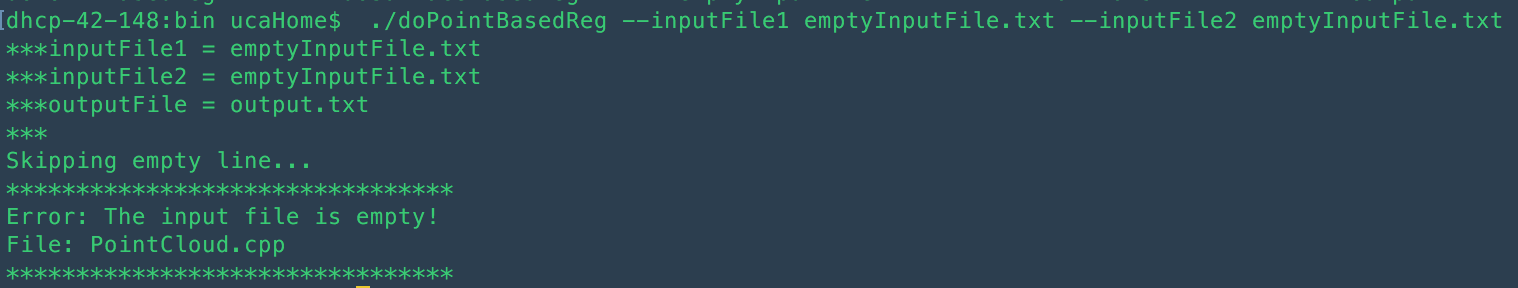
\includegraphics[width=\textwidth]{exception}%
\caption{Example of exception}
\label{fig:exceptionEx}
\end{figure*}
%%%%%%%%%%%%%%%%%%%%%%%%%%%%%%%%%%%%%%%%

Error checking:
\begin{itemize}
	\item the input files for point based registration have to have a single point per line (x y z)
	\item the input files for surface based registration have to have 3 points per line (x1 y1 z1 x2 y2 z2 x3 y3 z3)
	\item the constructor for PointCloud cannot be called with an empty point set
	\item exceptions are thrown if the $std::stringstream$ or the input streams  cannot be opened 
	\item the method $PointCloud::applyTransformation()$ checks that the input transformation is in the format $ T = [R | t] $
	\item the ICPRegistation solver checks if the two point clouds have the same size
\end{itemize}

The Catch library was used to implement unit testing on the ICP program (20 assertions in 6 test cases). The tests were structured in TEST\_CASE and SECTIONs, using positive (REQUIRE) and negative tests (REQUIRE\_THROWS). For the tests on Surface Based Registration, different input files were created with the same transformation matrix (with less points) to decrease the computation time.\\

Here is a list of some of the functions tested:
\begin{itemize}
	\item Point Cloud Class
	\begin{itemize}
		\item test whether the PointCloud class has correct methods - computes the mean correctly, it centers the point set correctly
		\item test whether the PointCloud class throws exceptions (negative tests) - empty point set, empty input file, invalid transformation, incorrect size of input point set
	\end{itemize}
	\item Point Based Registration
	\begin{itemize}
		\item test whether the PointBasedRegistration output is correct
		\item test the least squares estimation
		\item test whether the LS estimation throws an exception - unequal point set sizes
	\end{itemize}
	\item Surface Based Registration
	\begin{itemize}
		\item test whether the SurfaceBasedRegistration output is correct
		\item test the findCorrespondences method - whether it throws an exception - unequal point set sizes
		\item test the output of SurfaceBasedRegistration with identical matrices
	\end{itemize}
\end{itemize}

%%%%%%%%%%%%%%%%%%%%%%%%%%%%%%%%%%%%%%%%
\begin{figure*}[!h]
\centering
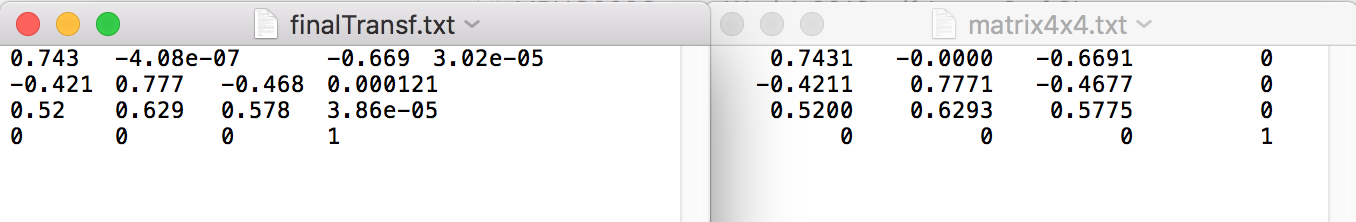
\includegraphics[width=\textwidth]{unitTestPBR}%
\caption{Point Based Registration: Left - Estimated transformation matrix; Right - Ground truth transformation matrix}
\label{fig:unitTestPBR}
\end{figure*}
%%%%%%%%%%%%%%%%%%%%%%%%%%%%%%%%%%%%%%%%


%%%%%%%%%%%%%%%%%%%%%%%%%%%%%%%%%%%%%%%%
\begin{figure*}[!h]
\centering
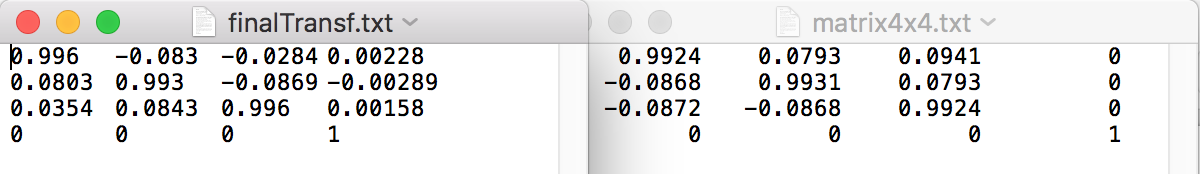
\includegraphics[width=\textwidth]{unitTestSBR}%
\caption{Surface Based Registration: Left - Estimated transformation matrix; Right - Ground truth transformation matrix}
\label{fig:unitTestPBR}
\end{figure*}
%%%%%%%%%%%%%%%%%%%%%%%%%%%%%%%%%%%%%%%%

The difference between the transformation matrices in the surface based case is bigger than in the least squares estimation. One solution would be to filter out the bad correspondences between the point sets. This could be done by thresholding the distance between them, or comparing their normals.\\

Most of the test cases implemented use fixtures to test if the estimated output is close enough to the ground truth. Moreover, they use a setup/teardown approach in which an object is created in the main TEST\_CASE and different scenarios are tested in individual SECTIONS. The type of testing done in this project is closer to Behaviour Driven Development. Each test was created to check for errors that might be caused from the end-user perspective.

\end{homeworkProblem}
\clearpage

%----------------------------------------------------------------------------------------
%----------------------------------------------------------------------------------------
%	PROBLEM 3
%----------------------------------------------------------------------------------------

\begin{homeworkProblem}

\textbf{Connect all the components together - Point Based Registration}\\

The Boost library was used to create entry points for the Point Based and Surface Based Registration. Their robust implementation of command line parsing allows specifying default and implicit values, positional and optional arguments and descriptions for the different flags.\\

The argument $-e/--example$ was added to illustrate a call to the program. The files provided in the testing folders are used as input. The output is written to a text file by default.

%%%%%%%%%%%%%%%%%%%%%%%%%%%%%%%%%%%%%%%%
\begin{figure*}[!h]
\centering
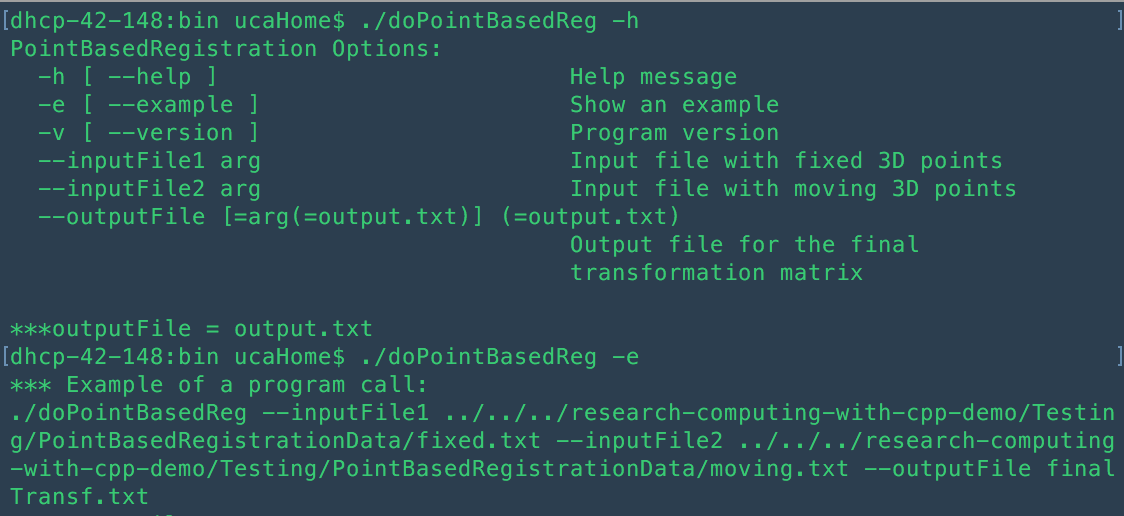
\includegraphics[width=\textwidth]{pbr_entrypoint}%
\caption{Point Based Registration - Command line entry point and example of a call}
\label{fig:entrypoint_pbr}
\end{figure*}
%%%%%%%%%%%%%%%%%%%%%%%%%%%%%%%%%%%%%%%%

\end{homeworkProblem}
\clearpage

%----------------------------------------------------------------------------------------
%----------------------------------------------------------------------------------------
%	PROBLEM 4
%----------------------------------------------------------------------------------------
\begin{homeworkProblem}
  
\textbf{Connect all the components together - Surface Based Registration}\\

The Surface Based Registration entry point is structured in a similar way to Point Based Registration. The example calls the function with the text files in the testing folder.

%%%%%%%%%%%%%%%%%%%%%%%%%%%%%%%%%%%%%%%%
\begin{figure*}[!h]
\centering
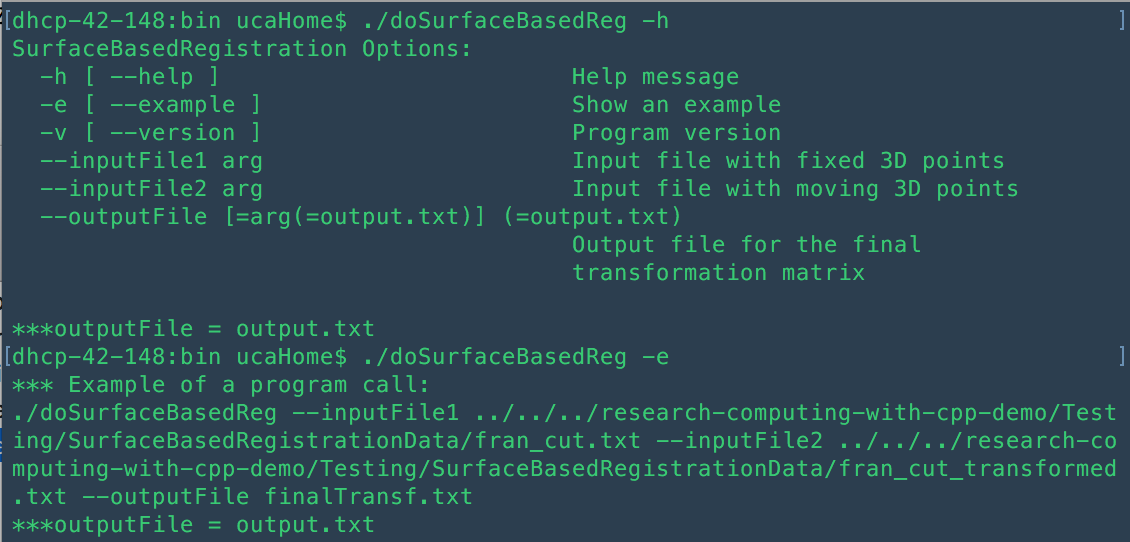
\includegraphics[width=\textwidth]{sbr_entrypoint}%
\caption{Surface Based Registration - Command line entry point and example of a call}
\label{fig:entrypoint_sbr}
\end{figure*}
%%%%%%%%%%%%%%%%%%%%%%%%%%%%%%%%%%%%%%%%

\end{homeworkProblem}
\clearpage
%----------------------------------------------------------------------------------------
%----------------------------------------------------------------------------------------
%	PROBLEM 5
%----------------------------------------------------------------------------------------
\begin{homeworkProblem}
    
\textbf{Medical Imaging application}\\

The slowest part of the current algorithm is the correspondence step. In this implementation, a naive approach is taken where for each point, the closest point is found by computing all the distances between the two point sets. This step could be significantly improved in order to speed up the process. One approach would be to store the data points in a kd-tree. This way, the search of the pair would be much faster. Libraries like ANN or FASTANN implement approximate nearest neighbour algorithms based on kd-trees efficiently. With this approach, more neighbouring points could be found. The pair could be selected based on additional criteria other than the distance, like the orientation of the normals or the colour/texture of the mesh.

\end{homeworkProblem}


%----------------------------------------------------------------------------------------
%\afterpage{\blankpage}
%\clearpage
%\bibliographystyle{ieeetr}
%\bibliography{ap3dgLIB}

\end{document}}